\chapter{Aberration Correction in for Spinning Disk Confocal Microscopy}
\label{chpt:Aurox}

\section{Image Formation in Aurox Clarity Module}
\label{sec:Aurox_image_formation}

Figure~\ref{fig:confocal_schematic} shows a simplified schematic for a Nipkow-Petran spinning disk confocal microscope. The excitation illumination passes through aperture mask, which is then imaged onto the sample. This aperture mask consists of a number of pinholes packed closely together, illumating a number of focal spots at once. The excitation light then passes back through the aperture mask where the out-of-focus light is discarded by the pinhole array.\cite{egger1967new,fuseler2018types}

\begin{figure}[h]
	\centering
	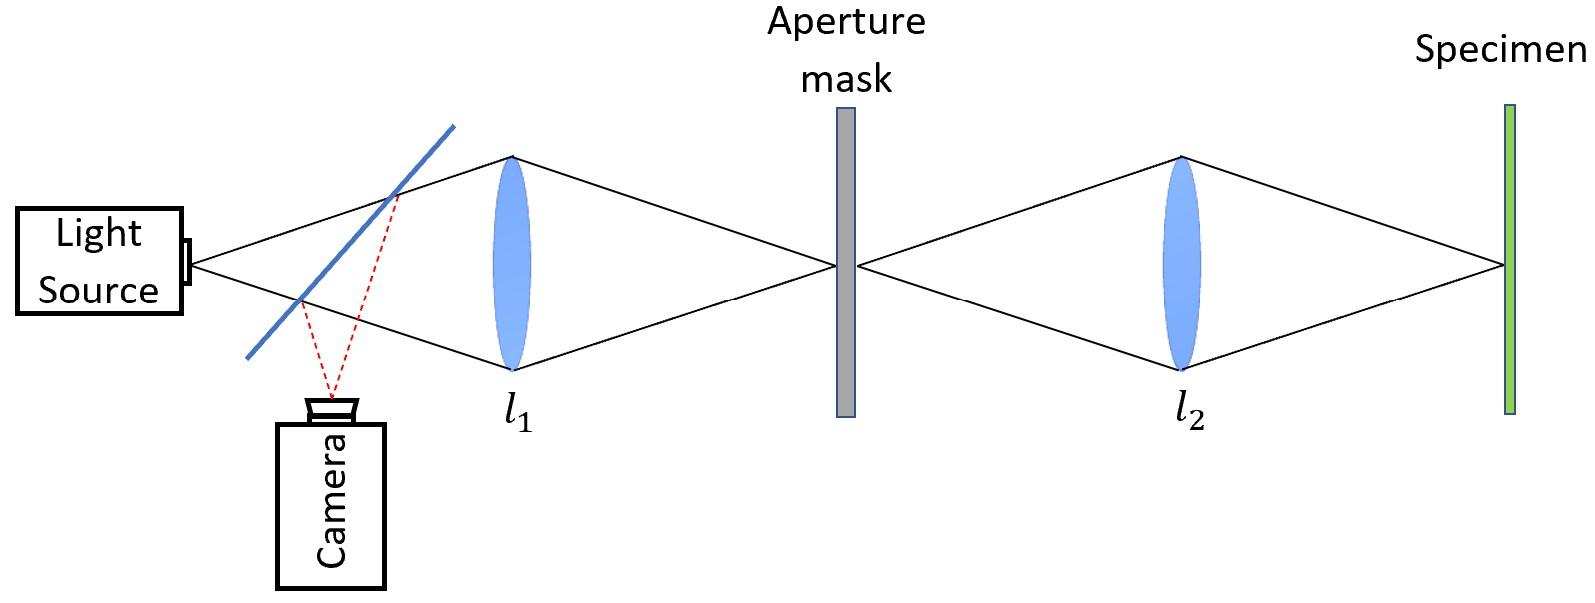
\includegraphics[width=\textwidth]{images/confocal_schematic.jpg}
	\caption{A schematic diagram showing a simplified layout for a Nipkow-Petran spinning disk confocal microscope}
	\label{fig:confocal_schematic}
\end{figure}

Consider a transmissive optical system as shown in Figure~\ref{fig:optical_system_schematic}. For an incoherent light source, immediately after the detector mask the intensity, $I\left(\textbf{x}_{2}\right)$, is given by:

\begin{equation}\label{eq:intensity_after_detector}
	I\left(\textbf{x}_{2}\right) = \int S\left(\textbf{x}_{1}\right) D\left(\textbf{x}_{2}\right) \left| \int h_{1}\left(\textbf{x}_{0} + \frac{\textbf{x}_{1}}{M}\right) \tau\left(\textbf{x}_{0}\right) h_{2}\left(\textbf{x}_{0} + \frac{\textbf{x}_{2}}{M}\right)d\textbf{x}_{0}\right|^{2}d\textbf{x}_{1}
\end{equation}

Where $S\left(\textbf{x}_{1}\right)$ is the intensity sensitivity of the source mask, $D\left(\textbf{x}_{2}\right)$ is the detector mask, $\tau\left(\textbf{x}_{0}\right)$ is the amplitude transmittance function of the aperture mask, $h_{1}$ and $h_{2}$ are the amplitude point spread functions (PSFs) of the two imaging lenses respectively and $M$ is the magnification factor. 

\begin{figure}[h]
	\centering
	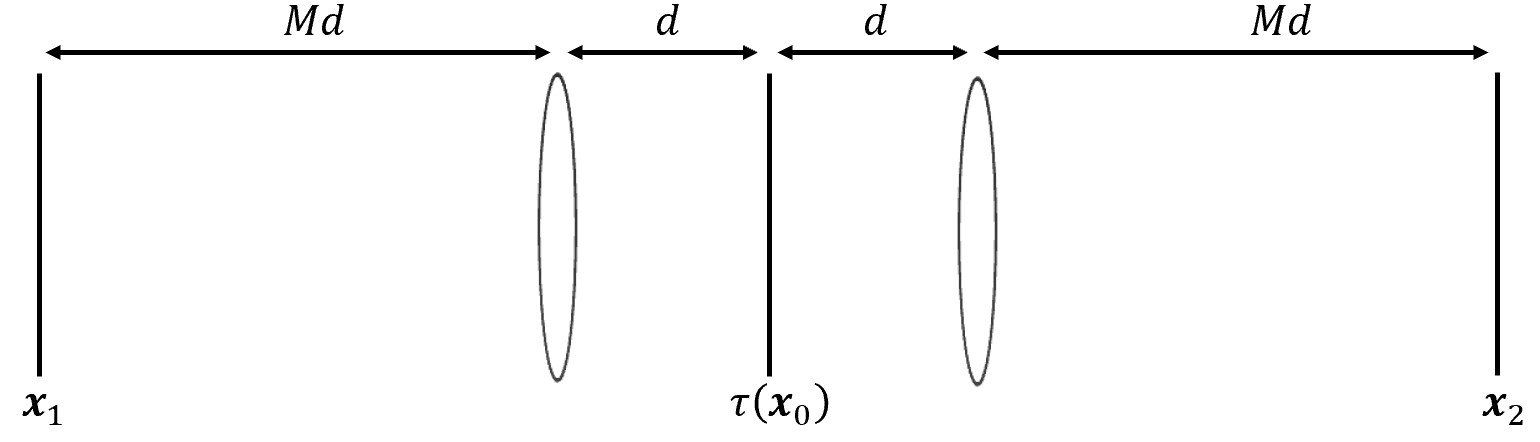
\includegraphics[width=\textwidth]{images/optical_system_schematic.jpg}
	\caption{A simple schematic diagram of a transmissive optical system}
	\label{fig:optical_system_schematic}
\end{figure}

Consider the case of reflection just after the detector mask and with the detector aperture positioned at some $\textbf{x}_{i}$ such that $S\left(\textbf{x}\right) = D\left(\textbf{x}\right) = \delta\left(\textbf{x} - \textbf{x}_{i}\right)$, where here $\delta$ denotes the Dirac delta function. In this case, assuming an ideal point source, the intensity at $\textbf{x}_{i}$ from Equation~\ref{eq:intensity_after_detector} becomes:

\begin{equation}\label{eq:confocal_image_form}
	I\left(\textbf{x}_{i}\right) = \left| \int h_{1}\left(\textbf{x}\right) h_{2}\left(\textbf{x}\right) \tau\left(\textbf{x} - \frac{\textbf{x}_{i}}{M}\right)d\textbf{x}\right|^{2}
\end{equation}

Which is the equation which describes image formation in conventional confocal microscopes.\cite{wilson1990confocal} This describes the image formation from a single point source and hence requires scanning in $\textbf{x}_{i}$ to form a complete image of the field of view of the object. To remove the need for scanning, the source and detector masks should instead be composed of an array of pixels with variable transmittence where each pixel's transmittence is time dependent, $b_{i}\left(t\right)$. The source and detector masks can then be described by:

\begin{equation}\label{eq:detector_aperture_time}
	S\left(\textbf{x}\right) = D\left(\textbf{x}\right) = \sum_{i=0}^{N} b_{i}\left(t\right)\delta\left(\textbf{x} - \textbf{x}_{i}\right)
\end{equation}

Where $N$ is the number of pixels and each pixel has a coordinate $\textbf{x}_{1}, \textbf{x}_{2},...,\textbf{x}_{N}$. The resultant image is given by the time average of Equation~\ref{eq:intensity_after_detector}:

\begin{equation}\label{eq:confocal_image_time_ave}
	\left\langle I\left(\textbf{x}_{2}\right)\right\rangle = \left\langle \int S\left(\textbf{x}_{1}\right) D\left(\textbf{x}_{2}\right) \left| \int h_{1}\left(\textbf{x}_{0} + \frac{\textbf{x}_{1}}{M}\right) \tau\left(\textbf{x}_{0}\right) h_{2}\left(\textbf{x}_{0} + \frac{\textbf{x}_{2}}{M}\right)d\textbf{x}_{0}\right|^{2}d\textbf{x}_{1}\right\rangle
\end{equation}

Where $\left\langle . \right\rangle$ is the time average. Since the only time-dependent components are $S\left(\textbf{x}_{1}\right)$ and $D\left(\textbf{x}_{2}\right)$ only the time average of $S\left(\textbf{x}_{1}\right) D\left(\textbf{x}_{2}\right)$ need be considered:

\begin{equation}\label{eq:SD_time_ave}
	\left\langle S\left(\textbf{x}_{1}\right) D\left(\textbf{x}_{2}\right)\right\rangle = \sum_{i=0}^{N}\sum_{j=0}^{N} \left\langle b_{i}\left(t\right) b_{j}\left(t\right)\right\rangle \delta\left(\textbf{x}_{1} - \textbf{x}_{i}\right) \delta\left(\textbf{x}_{2} - \textbf{x}_{j}\right)
\end{equation}

The transmittence of each pixel should be entirely uncorreleted with the transmittence of any other pixel. Therefore, a sequence of transmittences is chosen such that:

\begin{equation}\label{eq:pixel_uncorrelation}
	\left\langle b_{i}\left(t\right) b_{j}\left(t\right)\right\rangle = \delta_{ij}
\end{equation}

Where $\delta_{ij}$ is the Kronecker delta. $b_{i}\left(t\right)$ can therefore be any orthonormal sequence, such as an infinite, random sequence of $\pm1$ or finite-length complementary Golay sequences.\cite{golay1949multi} Unfortunately, such sequences require negative transmittence values which is optically achievable. By adding a DC shift this limitation can be overcome and the pixel transmissivities become:

\begin{equation}\label{eq:detector_aperture_time_DC}
	S\left(\textbf{x}\right) = D\left(\textbf{x}\right) = \frac{1}{2} \sum_{i=0}^{N} \left[b_{i}\left(t\right) + 1\right]\delta\left(\textbf{x} - \textbf{x}_{i}\right)
\end{equation} 

So the pixel transmissivities, $\left[b_{i}\left(t\right) + 1\right]$, alternate between $0$ and $1$ as $b_{i}\left(t\right)$ varies between $\pm1$. Imposing the additional requirement that $\left\langle b_{i}\left(t\right) \right\rangle = 0$, then Equation~\ref{eq:SD_time_ave} becomes:

\begin{equation}\label{eq:SD_time_ave_DC}
	\begin{split}
		\left\langle S\left(\textbf{x}_{1}\right) D\left(\textbf{x}_{2}\right)\right\rangle &= \frac{1}{4} \sum_{i=0}^{N}\sum_{j=0}^{N} \left\langle \left[b_{i}\left(t\right) + 1\right] \left[b_{j}\left(t\right) + 1\right] \right\rangle \delta\left(\textbf{x}_{1} - \textbf{x}_{i}\right) \delta\left(\textbf{x}_{2} - \textbf{x}_{j}\right)\\
		&= \frac{1}{4} \left[\sum_{i=0}^{N} \delta\left(\textbf{x}_{1} - \textbf{x}_{i}\right) \delta\left(\textbf{x}_{2} - \textbf{x}_{i}\right) + \sum_{i=0}^{N}\sum_{j=0}^{N} \delta\left(\textbf{x}_{1} - \textbf{x}_{i}\right) \delta\left(\textbf{x}_{2} - \textbf{x}_{j}\right)\right]\\
	\end{split}
\end{equation}

Substituting Equation~\ref{eq:SD_time_ave_DC} into Equation~\ref{eq:confocal_image_time_ave} yeilds two terms. The first term is the same form as Equation~\ref{eq:confocal_image_form} i.e. a conventional confocal image. The second term is a non-confocal image where all the pixel transmissivities are the same. At the limit, where all pixels are adjacent and there is no space inbetween them, then $S\left(\textbf{x}\right) = D\left(\textbf{x}\right) = \Sigma_{i=1}^{N}\delta\left(\textbf{x} - \textbf{x}_{i}\right) = 1$ i.e. a purely conventional image.\cite{juskaitis1996efficient,wilson1996confocal}. Therefore the image formed by the transmitted light, $I_{T}$, is a composite of a conventional and confocal image:

\begin{equation}\label{eq:transmitted_image}
	I_{T} = I_{conf} + I_{conv}
\end{equation}

Where $I_{conf}$ and $I_{conv}$ are the confocal and conventional images respectively. Instead of an array of pixels with programmable transmissivity, the Aurox Clarity module implements a disk with a photolithographed transmittence sequence. In this case, the transmittence pattern presented to a given fixed pixel is equivalent to the transmittence pattern along the corresponding arc of the disk.\cite{wilson1996confocal} Equation~\ref{eq:detector_aperture_time_DC} should therefore be modified to:

\begin{equation}\label{eq:detector_aperture_arc}
S\left(\textbf{x}\right) = D\left(\textbf{x}\right) = \frac{1}{2} \sum_{i=0}^{N} \left[b_{i}\left(\textbf{x}_{r}\right) + 1\right]\delta\left(\textbf{x} - \textbf{x}_{i}\right)
\end{equation}

Where $\textbf{x}_{r}$ is the rotation coordinate. In this case, the final image is obtained by averaging over $\textbf{x}_{r}$ rather than over time, but the result is still Equation~\ref{eq:transmitted_image}. Previous implementation of this approach acquired two images, the second of which had $b_{i}\left(\textbf{x}_{r}\right) = 1$ i.e. no aperture mask. As Figure~\ref{fig:aurox_clarity_internal} shows, the Aurox clarity module images both the light transmitted through the spinning disk and the light reflected off the disk where the transmissivity is $0$. In this case, the aperture mask is defined as:

\begin{equation}\label{eq:detector_aperture_arc_reflect}
	S\left(\textbf{x}\right) = D\left(\textbf{x}\right) = \frac{1}{2} \sum_{i=0}^{N} \left[1 - b_{i}\left(\textbf{x}_{r}\right)\right]\delta\left(\textbf{x} - \textbf{x}_{i}\right)
\end{equation}

Applying the same average over $\textbf{x}_{r}$ as before, the image formed by the reflected light, $I_{R}$, is:

\begin{equation}\label{eq:reflected_image}
	I_{R} = I_{conv} - I_{conf}
\end{equation}

Therefore, both the confocal and conventional images can be recovered by:

\begin{equation}\label{eq:confocal_image}
	I_{conf} = \frac{1}{2}\left(I_{T} - I_{R}\right)
\end{equation}

\begin{equation}\label{eq:conventional_image}
I_{conv} = \frac{1}{2}\left(I_{T} + I_{R}\right)
\end{equation}

This has the benefits of only requiring one exposure for the sample to acquire a confocal image and using all of the emitted fluorescence light.

	\subsection{Aberrations and Image Formation}
	\label{subsec:Aurox_aberrations}

\section{Biological Exemplar}
\label{sec:Aurox_biology}

	\begin{itemize}
		\item Explain why the particular sample needs the correction provided, what you can't normally resolve without AO and show how  AO improves it.
	\end{itemize}

	\subsection{Sample preperation}
	\label{subsec:Aurox_sample_prep}
	
\section{Experimental Results}
\label{sec:Aurox_results}
